\section{Durchführung}
\label{sec:Durchführung}
In der ersten Messreihe werden fünf Kennlinien aufgenommen, dazu wird die Heizstrom von $2,5\si{\ampere}$ bis $2,1\si{\ampere}$
in $0,1\si{\volt}$ Schritten eingestellt. Für jede Heizstromseinstellung wird die Spannung von $0-250\si{\volt}$ hochgeregelt,
zuerst in $5\si{\volt}$-Schritten und ab $60\si{\volt}$ in $10\si{\volt}$-Schritten,
der entsprechende Strom wird notiert. Der Aufbau ist in Abbildung \ref{fig:aufbau1} zu finden.
\begin{figure}
 \centering
 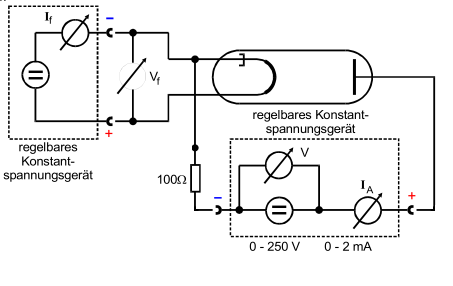
\includegraphics[width=0.5\textwidth]{Aufbaukenn.png}
 \caption{Aufbau zur Aufnahme der Kennlinien.\cite{sample}}
 \label{fig:aufbau1}
 \end{figure}

Bei der anschließenden Messung wird der Anlaufstrom vermessen. Bei maximalem Heizstrom wird eine Gegenspannung angelegt und
in $0,05\si{\volt}$-Schritten bis $1\si{\volt}$ hochgeregelt, der entsprecheende Anlaufstrom wird registrieert.
Die Abbildung \ref{fig:aufbau2} enthält den benötigten Aufbau.
\begin{figure}
 \centering
 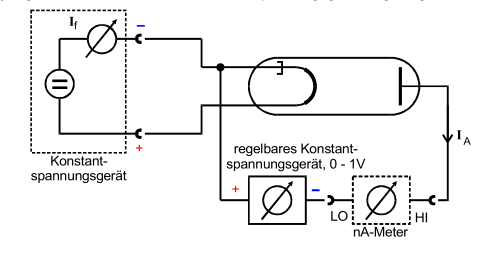
\includegraphics[width=0.5\textwidth]{Aufbauan.png}
 \caption{Aufbau zur Aufnahme der Anlaufstromkurve.\cite{sample}}
 \label{fig:aufbau2}
 \end{figure}
